\documentclass[12pt,a4paper]{article}
\usepackage{amsmath}
\usepackage{amssymb}
\usepackage{amsfonts}
\usepackage{amsthm}  % Added for theorem environments
\usepackage{bm}
\usepackage{graphicx}
\usepackage{geometry}
\geometry{margin=1in}
\usepackage{tikz}
\usepackage{algorithm}
\usepackage{algorithmic}
\usepackage{tikz}
\usetikzlibrary{3d,calc}
\usetikzlibrary{arrows.meta,decorations.pathreplacing}
\usetikzlibrary{shapes,positioning}
\usetikzlibrary{backgrounds}
\usetikzlibrary{patterns}
\usetikzlibrary{matrix}
\usetikzlibrary{fit}
\usetikzlibrary{shadows}
\usetikzlibrary{angles,quotes}
\usetikzlibrary{babel}

% Define theorem environments
\newtheorem{definition}{Definition}[section]
\newtheorem{theorem}{Theorem}[section]
\newtheorem{lemma}{Lemma}[section]

\title{Cross-Correlation Coefficient for Electron Density Map Fitting:
Mathematical Framework and Implementation}
\author{Analysis of IMP Electron Microscopy Module}
\date{}

\begin{document}

\maketitle

\section{Introduction}

The cross-correlation coefficient (CCC) is a fundamental metric 
used in computational structural biology to quantify the similarity 
between experimental electron density maps and theoretical model-derived 
density maps. This document presents the mathematical framework underlying 
the coarse cross-correlation fitting methodology used in molecular structure 
refinement against cryo-electron microscopy data.

\section{Theoretical Foundation}
\subsection{Three-Dimensional Density Representation}

Electron density maps represent the spatial distribution of 
electron probability in three-dimensional space. Mathematically, 
the electron density $\rho(\mathbf{r})$ is a scalar field defined 
over continuous 3D space, where $\mathbf{r} = (x, y, z)$ represents 
a position vector.

In computational implementations, this continuous density field 
must be discretized onto a regular three-dimensional grid. This 
discretization process transforms the continuous function 
$\rho(\mathbf{r})$ into a discrete array $\rho_{i,j,k}$, where 
indices $(i,j,k)$ correspond to grid points in the $x$, $y$, and $z$ 
directions, respectively.

\subsubsection{From Pixels to Voxels}

In two-dimensional image processing, the fundamental unit of 
discretization is the \textit{pixel} (picture element), which 
represents a square region in the $(x,y)$ plane with uniform 
intensity. Each pixel occupies an area:

\begin{equation}
A_{pixel} = \Delta x \cdot \Delta y
\end{equation}

where $\Delta x$ and $\Delta y$ are the pixel dimensions 
along the respective axes.

The three-dimensional generalization of a pixel is a 
\textit{voxel} (volume element), which represents a cubic 
or rectangular parallelepiped region in 3D space. Each voxel 
occupies a volume:

\begin{equation}
V_{voxel} = \Delta x \cdot \Delta y \cdot \Delta z
\end{equation}

where $\Delta x$, $\Delta y$, and $\Delta z$ are the voxel 
dimensions along the three coordinate axes.

\subsubsection{Mathematical Grid Representation}

The discretized density map can be represented as a 
three-dimensional array with dimensions $N_x \times N_y \times N_z$, 
where each element $\rho_{i,j,k}$ corresponds to the average density 
within voxel $(i,j,k)$:

\begin{equation}
\rho_{i,j,k} = \frac{1}{V_{voxel}} \int_{x_i}^{x_i + \Delta x} \int_{y_j}^{y_j + \Delta y} \int_{z_k}^{z_k + \Delta z} \rho(x,y,z) \, dx \, dy \, dz
\end{equation}

The relationship between grid indices and physical coordinates is given by:

\begin{align}
x_i &= x_{origin} + i \cdot \Delta x \\
y_j &= y_{origin} + j \cdot \Delta y \\
z_k &= z_{origin} + k \cdot \Delta z
\end{align}

where $(x_{origin}, y_{origin}, z_{origin})$ defines the coordinate system origin.

\begin{figure}[h]
\centering
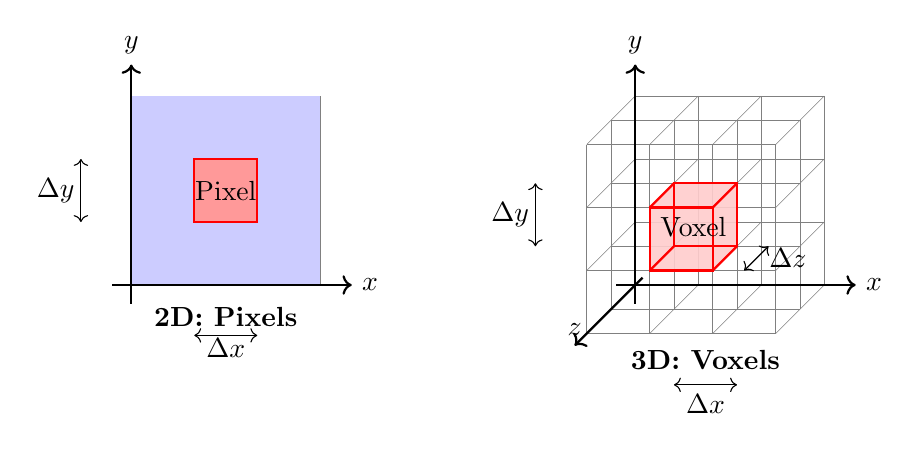
\begin{tikzpicture}[scale=0.8]
    % 2D pixel representation
    \begin{scope}[xshift=-4cm]
        \draw[step=1cm,gray,very thin] (0,0) grid (3,3);
        \foreach \x in {0,1,2}
            \foreach \y in {0,1,2}
                \fill[blue!20] (\x,\y) rectangle (\x+1,\y+1);
        
        % Highlight one pixel
        \fill[red!40] (1,1) rectangle (2,2);
        \draw[red,thick] (1,1) rectangle (2,2);
        
        % Labels
        \node at (1.5,1.5) {Pixel};
        \node at (1.5,-0.5) {\textbf{2D: Pixels}};
        
        % Axes
        \draw[->,thick] (-0.3,0) -- (3.5,0) node[right] {$x$};
        \draw[->,thick] (0,-0.3) -- (0,3.5) node[above] {$y$};
        
        % Dimensions
        \draw[<->] (1,-0.8) -- (2,-0.8);
        \node at (1.5,-1) {$\Delta x$};
        \draw[<->] (-0.8,1) -- (-0.8,2);
        \node at (-1.2,1.5) {$\Delta y$};
    \end{scope}
    
    % 3D voxel representation
    \begin{scope}[xshift=4cm]
        % Draw 3D grid structure
        \foreach \z in {0,1,2} {
            \begin{scope}[canvas is xy plane at z=\z]
                \draw[step=1cm,gray,very thin] (0,0) grid (3,3);
            \end{scope}
        }
        
        % Vertical lines
        \foreach \x in {0,1,2,3}
            \foreach \y in {0,1,2,3}
                \draw[gray,very thin] (\x,\y,0) -- (\x,\y,2);
        
        % Highlight one voxel
        \fill[red!20,opacity=0.7] (1,1,1) -- (2,1,1) -- (2,2,1) -- (1,2,1) -- cycle;
        \fill[red!20,opacity=0.7] (1,1,2) -- (2,1,2) -- (2,2,2) -- (1,2,2) -- cycle;
        \fill[red!20,opacity=0.7] (1,1,1) -- (1,2,1) -- (1,2,2) -- (1,1,2) -- cycle;
        \fill[red!20,opacity=0.7] (2,1,1) -- (2,2,1) -- (2,2,2) -- (2,1,2) -- cycle;
        \fill[red!20,opacity=0.7] (1,1,1) -- (2,1,1) -- (2,1,2) -- (1,1,2) -- cycle;
        \fill[red!20,opacity=0.7] (1,2,1) -- (2,2,1) -- (2,2,2) -- (1,2,2) -- cycle;
        
        \draw[red,thick] (1,1,1) -- (2,1,1) -- (2,2,1) -- (1,2,1) -- cycle;
        \draw[red,thick] (1,1,2) -- (2,1,2) -- (2,2,2) -- (1,2,2) -- cycle;
        \draw[red,thick] (1,1,1) -- (1,1,2);
        \draw[red,thick] (2,1,1) -- (2,1,2);
        \draw[red,thick] (1,2,1) -- (1,2,2);
        \draw[red,thick] (2,2,1) -- (2,2,2);
        
        \node at (1.5,1.5,1.5) {Voxel};
        \node at (1.5,-0.8,1) {\textbf{3D: Voxels}};
        
        % Axes
        \draw[->,thick] (-0.3,0,0) -- (3.5,0,0) node[right] {$x$};
        \draw[->,thick] (0,-0.3,0) -- (0,3.5,0) node[above] {$y$};
        \draw[->,thick] (0,0,-0.3) -- (0,0,2.5) node[above] {$z$};
        
        % Dimensions
        \draw[<->] (1,-1.2,1) -- (2,-1.2,1);
        \node at (1.5,-1.5,1) {$\Delta x$};
        \draw[<->] (-1.2,1,1) -- (-1.2,2,1);
        \node at (-1.6,1.5,1) {$\Delta y$};
        \draw[<->] (2.5,1,1) -- (2.5,1,2);
        \node at (3,1,1.5) {$\Delta z$};
    \end{scope}
\end{tikzpicture}
\caption{Discretization of continuous space into discrete 
elements: (left) 2D pixels with area $\Delta x \times \Delta y$, 
and (right) 3D voxels with volume $\Delta x \times \Delta y \times \Delta z$. 
Each element stores a single density value representing the average 
density within that spatial region.}
\label{fig:pixel_voxel}
\end{figure}

\subsubsection{Linear Indexing}

For computational efficiency, the three-dimensional voxel array 
is often stored in memory using a linear indexing scheme. The 
conversion between 3D indices $(i,j,k)$ and a linear index $\ell$ 
is given by:

\begin{equation}
\ell = k \cdot N_x \cdot N_y + j \cdot N_x + i
\end{equation}

This linear indexing is crucial for efficient memory access patterns 
and is used extensively in the cross-correlation calculations described 
in subsequent sections.
\subsection{Cross-Correlation Coefficient Definition}

The cross-correlation coefficient between two density maps 
$\rho_1(\mathbf{r})$ and $\rho_2(\mathbf{r})$ is defined as:

\begin{equation}
CCC = \frac{\sum_{\mathbf{r}} (\rho_1(\mathbf{r}) - \langle\rho_1\rangle)(\rho_2(\mathbf{r}) - \langle\rho_2\rangle)}{\sqrt{\sum_{\mathbf{r}} (\rho_1(\mathbf{r}) - \langle\rho_1\rangle)^2 \sum_{\mathbf{r}} (\rho_2(\mathbf{r}) - \langle\rho_2\rangle)^2}}
\end{equation}

where $\langle\rho_i\rangle$ represents the mean density value 
of map $i$, and the summation extends over all voxels $\mathbf{r}$ 
in the density grid.

\subsection{Discrete Voxel Implementation}

For discretized density maps on a regular grid with $N$ voxels, 
the correlation coefficient becomes:

\begin{equation}
CCC = \frac{\sum_{i=1}^{N} (\rho_{1,i} - \bar{\rho_1})(\rho_{2,i} - \bar{\rho_2})}{N \cdot \sigma_{\rho_1} \cdot \sigma_{\rho_2}}
\end{equation}

where:
\begin{align}
\bar{\rho_j} &= \frac{1}{N}\sum_{i=1}^{N} \rho_{j,i} \quad \text{(mean density)} \\
\sigma_{\rho_j} &= \sqrt{\frac{1}{N}\sum_{i=1}^{N} (\rho_{j,i} - \bar{\rho_j})^2} \quad \text{(RMS density)}
\end{align}

\subsection{Threshold-Based Correlation}

To focus the correlation calculation on regions of significant 
density, a threshold-based approach is employed:

\begin{equation}
CCC_{thresh} = \frac{\sum_{i \in \Omega} \rho_{1,i} \rho_{2,i} - N_{thresh} \bar{\rho_1} \bar{\rho_2}}{N_{thresh} \sigma_{\rho_1} \sigma_{\rho_2}}
\end{equation}

where $\Omega = \{i : \rho_{2,i} > \tau\}$ is the set of voxels 
exceeding threshold $\tau$, and $N_{thresh} = |\Omega|$ is the 
number of such voxels.

\section{Spatial Alignment and Origin Handling}

\subsection{Same Origin Case}

When both density maps share the same coordinate origin, the 
correlation simplifies to a direct voxel-by-voxel comparison:

\begin{equation}
CCC_{same} = \frac{\sum_{i=1}^{N} \mathbb{I}(\rho_{2,i} > \tau) \rho_{1,i} \rho_{2,i}}{\sum_{i=1}^{N} \mathbb{I}(\rho_{2,i} > \tau)}
\end{equation}

where $\mathbb{I}(\cdot)$ is the indicator function.

\subsection{Different Origins Case}

When density maps have different coordinate origins, a spatial 
transformation is required. The voxel index transformation is:

\begin{equation}
j = i + \Delta_{shift}
\end{equation}

where the shift parameter is calculated as:

\begin{equation}
\Delta_{shift} = \Delta z \cdot n_x \cdot n_y + \Delta y \cdot n_x + \Delta x
\end{equation}

with voxel offsets:
\begin{align}
\Delta x &= \lfloor \frac{x_{origin,2} - x_{origin,1}}{v_{size}} \rfloor \\
\Delta y &= \lfloor \frac{y_{origin,2} - y_{origin,1}}{v_{size}} \rfloor \\
\Delta z &= \lfloor \frac{z_{origin,2} - z_{origin,1}}{v_{size}} \rfloor
\end{align}

where $v_{size}$ is the voxel size and $n_x, n_y$ are the grid dimensions.

\section{Local Cross-Correlation}

\subsection{Adaptive Mean and RMS Calculation}

For local correlation analysis, the mean and RMS values are 
computed only over the threshold-exceeding region:

\begin{align}
\bar{\rho}_{1,local} &= \frac{1}{N_{thresh}} \sum_{i \in \Omega} \rho_{1,j+i} \\
\bar{\rho}_{2,local} &= \frac{1}{N_{thresh}} \sum_{i \in \Omega} \rho_{2,i}
\end{align}

\begin{align}
\sigma_{1,local} &= \sqrt{\frac{1}{N_{thresh}} \sum_{i \in \Omega} (\rho_{1,j+i} - \bar{\rho}_{1,local})^2} \\
\sigma_{2,local} &= \sqrt{\frac{1}{N_{thresh}} \sum_{i \in \Omega} (\rho_{2,i} - \bar{\rho}_{2,local})^2}
\end{align}

\subsection{Local Correlation Coefficient}

The local cross-correlation coefficient is then:

\begin{equation}
CCC_{local} = \frac{\sum_{i \in \Omega} (\rho_{1,j+i} - \bar{\rho}_{1,local})(\rho_{2,i} - \bar{\rho}_{2,local})}{N_{thresh} \cdot \sigma_{1,local} \cdot \sigma_{2,local}}
\end{equation}

\section{Scoring Function}

\subsection{Coarse Correlation Score}

The final scoring function converts the correlation coefficient 
to an energy-like term:

\begin{equation}
E_{score} = \lambda (1 - CCC)
\end{equation}

where $\lambda$ is a scaling factor that determines the relative 
weight of the correlation term in the overall energy function.

\subsection{Normalization Factors}

When external normalization factors are provided, the correlation is adjusted as:

\begin{equation}
CCC_{norm} = \frac{CCC_{raw} - \alpha}{\beta}
\end{equation}

where $\alpha$ and $\beta$ are pre-computed normalization parameters 
that account for systematic biases in the density comparison.

\section{Gradient Calculation for Optimization}

\subsection{Derivative Framework}

For molecular dynamics or Monte Carlo optimization, the gradient of 
the correlation score with respect to particle coordinates is required. 
The derivative of the correlation coefficient with respect to particle 
position $\mathbf{r}_k$ is:

\begin{equation}
\frac{\partial CCC}{\partial \mathbf{r}_k} = \frac{2 w_k \kappa_{norm}}{\lambda N \sigma_{\rho_1} \sigma_{\rho_2}} \sum_{i} \rho_{1,i} \nabla_{\mathbf{r}_k} K(\mathbf{r}_i - \mathbf{r}_k)
\end{equation}

\subsection{Gaussian Kernel Derivative}

Using a Gaussian kernel for density representation:

\begin{equation}
K(\mathbf{r}) = \exp\left(-\frac{|\mathbf{r}|^2}{2\sigma^2}\right)
\end{equation}

The gradient becomes:

\begin{equation}
\nabla_{\mathbf{r}_k} K(\mathbf{r}_i - \mathbf{r}_k) = \frac{(\mathbf{r}_k - \mathbf{r}_i)}{\sigma^2} K(\mathbf{r}_i - \mathbf{r}_k)
\end{equation}

\subsection{Final Derivative Expression}

The complete derivative for particle $k$ in direction $\alpha$ is:

\begin{equation}
\frac{\partial E_{score}}{\partial r_{k,\alpha}} = \frac{2 w_k \lambda \kappa_{norm}}{\sigma^2 N \sigma_{\rho_1} \sigma_{\rho_2}} \sum_{i \in BB(k)} \rho_{1,i} (r_{k,\alpha} - r_{i,\alpha}) K(\mathbf{r}_i - \mathbf{r}_k)
\end{equation}

where $BB(k)$ represents the local bounding box around 
particle $k$, and $w_k$ is the weight factor for particle $k$.

\section{Computational Considerations}

\subsection{Bounding Box Optimization}

To reduce computational complexity, derivatives are calculated 
only within a local bounding box of radius $R_{cut}$ around each 
particle, where:

\begin{equation}
R_{cut} = \alpha \sigma_{kernel}
\end{equation}

with $\alpha$ typically chosen as 3-4 to capture 99\% of the 
Gaussian kernel contribution.

\subsection{Threshold Sensitivity}

The choice of density threshold $\tau$ significantly affects 
the correlation calculation. Typically:

\begin{equation}
\tau = \rho_{min} + \epsilon
\end{equation}

where $\rho_{min}$ is the minimum density value and $\epsilon$ is 
a small positive constant to avoid numerical instabilities.

\section{Conclusion}

The cross-correlation coefficient provides a robust metric 
for comparing experimental and theoretical electron density 
maps in structural biology applications. The mathematical 
framework presented here enables efficient computation of 
both the correlation score and its derivatives, facilitating 
optimization of molecular structures against cryo-EM data through 
energy minimization or molecular dynamics simulations.

\section{Mathematical Foundations of Electron Microscopy Density Map Scoring in IMP: Introduction}
This document provides a comprehensive mathematical analysis of electron microscopy (EM) 
density map creation, comparison, and scoring as implemented in the Integrative Modeling Platform (IMP).

\section{Fundamental Concepts}

\subsection{Voxels and 3D Grids}
A \textbf{voxel} (volumetric pixel) is the 3D equivalent of a pixel, representing a value in a regular 3D grid.

\begin{definition}[Voxel]
A voxel at grid position $(i, j, k)$ represents a cubic volume element with:
\begin{itemize}
    \item Grid indices: $(i, j, k) \in \mathbb{Z}^3$ where $0 \leq i < n_x$, $0 \leq j < n_y$, $0 \leq k < n_z$
    \item World coordinates: $(x, y, z) \in \mathbb{R}^3$ 
    \item Density value: $\rho(i, j, k) \in \mathbb{R}$
\end{itemize}
\end{definition}

The transformation between grid indices and world coordinates:
\begin{equation}
\begin{pmatrix} x \\ y \\ z \end{pmatrix} = \begin{pmatrix} x_{\text{origin}} \\ y_{\text{origin}} \\ z_{\text{origin}} \end{pmatrix} + \begin{pmatrix} i \cdot v_s \\ j \cdot v_s \\ k \cdot v_s \end{pmatrix}
\end{equation}
where $v_s$ is the voxel size (spacing) in Angstroms.

\subsection{Density Maps}
A density map $D$ is a 3D scalar field:
\begin{equation}
D: \Omega \subset \mathbb{R}^3 \rightarrow \mathbb{R}
\end{equation}
where $\Omega$ is the spatial domain (bounding box).

\section{Model Density Map Creation}

\subsection{Coarse-Grained Model Representation}
A coarse-grained model consists of $N$ particles, each with:
\begin{itemize}
    \item Position: $\mathbf{r}_i = (x_i, y_i, z_i)$
    \item Radius: $R_i$
    \item Mass/Weight: $w_i = R_i^3$ (proportional to volume)
\end{itemize}

\subsection{Two-Step Density Generation Process}

\subsubsection{Step 1: Histogram Binning}
The initial density is created by binning particles into voxels:

\begin{equation}
\rho_0(\mathbf{v}) = \sum_{i=1}^{N} w_i \cdot \delta_{\text{voxel}}(\mathbf{r}_i, \mathbf{v})
\end{equation}

where $\delta_{\text{voxel}}(\mathbf{r}_i, \mathbf{v})$ is 1 if particle $i$ falls in voxel $\mathbf{v}$, and 0 otherwise.

In discrete form:
\begin{equation}
\rho_0(j, k, l) = \sum_{i=1}^{N} w_i \cdot \mathbb{1}_{[j,k,l]}(\mathbf{r}_i)
\end{equation}

where $\mathbb{1}_{[j,k,l]}$ is the indicator function for voxel $(j,k,l)$.

\subsubsection{Step 2: Gaussian Blurring}
The histogram is convolved with a Gaussian kernel to simulate resolution effects:

\begin{equation}
\rho_{\text{model}}(\mathbf{r}) = (\rho_0 * G_\sigma)(\mathbf{r})
\end{equation}

where the 3D Gaussian kernel is:
\begin{equation}
G_\sigma(\mathbf{r}) = \frac{1}{(2\pi\sigma^2)^{3/2}} \exp\left(-\frac{|\mathbf{r}|^2}{2\sigma^2}\right)
\end{equation}

\subsection{Resolution to Sigma Conversion}
The relationship between experimental resolution and Gaussian sigma:
\begin{equation}
\sigma = \frac{\text{resolution}}{2\sqrt{2\ln(2)}} \approx \frac{\text{resolution}}{2.355}
\end{equation}

This comes from the Full Width at Half Maximum (FWHM) relationship:
\begin{equation}
\text{FWHM} = 2\sqrt{2\ln(2)} \cdot \sigma
\end{equation}

\section{Experimental Density Map}
The experimental map $\rho_{\text{exp}}$ is obtained from cryo-EM reconstruction with:
\begin{itemize}
    \item Header information: dimensions $(n_x, n_y, n_z)$, origin, voxel size
    \item Density values at each voxel
    \item Resolution estimate
\end{itemize}

\section{Cross-Correlation Coefficient (CCC) Scoring}

\subsection{Standard Cross-Correlation}
The cross-correlation coefficient between experimental map $\rho_{\text{exp}}$ and model map $\rho_{\text{model}}$:

\begin{equation}
\text{CCC} = \frac{\sum_{\mathbf{v} \in \Omega} (\rho_{\text{exp}}(\mathbf{v}) - \bar{\rho}_{\text{exp}})(\rho_{\text{model}}(\mathbf{v}) - \bar{\rho}_{\text{model}})}{\sqrt{\sum_{\mathbf{v}} (\rho_{\text{exp}}(\mathbf{v}) - \bar{\rho}_{\text{exp}})^2} \sqrt{\sum_{\mathbf{v}} (\rho_{\text{model}}(\mathbf{v}) - \bar{\rho}_{\text{model}})^2}}
\end{equation}

where $\bar{\rho}$ denotes the mean density.

\subsection{Thresholded Cross-Correlation}
IMP uses a threshold to focus on significant density:

\begin{equation}
\text{CCC}_{\text{thresh}} = \frac{\sum_{\mathbf{v} \in \Omega_t} \rho_{\text{exp}}(\mathbf{v}) \cdot \rho_{\text{model}}(\mathbf{v}) - N_t \bar{\rho}_{\text{exp}} \bar{\rho}_{\text{model}}}{N_t \cdot \text{RMS}_{\text{exp}} \cdot \text{RMS}_{\text{model}}}
\end{equation}

where:
\begin{itemize}
    \item $\Omega_t = \{\mathbf{v} : \rho_{\text{model}}(\mathbf{v}) > \theta\}$ (thresholded region)
    \item $N_t = |\Omega_t|$ (number of voxels above threshold)
    \item $\theta$ is typically set to $\text{dmin}_{\text{model}} - \epsilon$
\end{itemize}

\subsection{Scoring Function}
The final score used for optimization:
\begin{equation}
S = \lambda \cdot (1 - \text{CCC})
\end{equation}
where $\lambda$ is a scale factor (typically positive), making the score minimize when CCC is maximized.

\section{Padding and Map Alignment}

\subsection{The Padding Problem}
When two maps have different dimensions or origins, direct comparison is not possible. Consider:
\begin{itemize}
    \item Map 1: dimensions $(n_{x1}, n_{y1}, n_{z1})$, origin $\mathbf{o}_1$
    \item Map 2: dimensions $(n_{x2}, n_{y2}, n_{z2})$, origin $\mathbf{o}_2$
\end{itemize}

\subsection{Padding Solution}
Padding creates expanded maps with unified dimensions:

\begin{algorithm}
\caption{Map Padding Algorithm}
\begin{algorithmic}
\STATE \textbf{Input:} Maps $D_1$, $D_2$ with different dimensions
\STATE \textbf{Output:} Padded maps $D_1'$, $D_2'$ with same dimensions
\STATE
\STATE 1. Compute merged bounding box:
\STATE \quad $\text{BB}_{\text{merged}} = \text{BB}(D_1) \cup \text{BB}(D_2)$
\STATE
\STATE 2. Create new dimensions:
\STATE \quad $n_x' = \max(n_{x1}, n_{x2})$
\STATE \quad $n_y' = \max(n_{y1}, n_{y2})$
\STATE \quad $n_z' = \max(n_{z1}, n_{z2})$
\STATE
\STATE 3. Create padded maps:
\STATE \quad $D_1'[i,j,k] = \begin{cases} D_1[i,j,k] & \text{if } (i,j,k) \in D_1 \\ 0 & \text{otherwise} \end{cases}$
\STATE \quad $D_2'[i,j,k] = \begin{cases} D_2[i,j,k] & \text{if } (i,j,k) \in D_2 \\ 0 & \text{otherwise} \end{cases}$
\end{algorithmic}
\end{algorithm}

\subsection{Mathematical Representation of Padding}
Padding can be represented as an embedding operation:
\begin{equation}
\iota: D \rightarrow D'
\end{equation}
where $D'$ is the padded space with:
\begin{equation}
D'(\mathbf{r}) = \begin{cases}
D(\mathbf{r}) & \text{if } \mathbf{r} \in \text{domain}(D) \\
0 & \text{otherwise}
\end{cases}
\end{equation}

\section{Box Dimensions and Bounding Boxes}

\subsection{Bounding Box Definition}
A bounding box $\text{BB}$ for a density map is defined by:
\begin{equation}
\text{BB} = [\mathbf{r}_{\min}, \mathbf{r}_{\max}] = [x_{\min}, x_{\max}] \times [y_{\min}, y_{\max}] \times [z_{\min}, z_{\max}]
\end{equation}

For a particle-based model:
\begin{align}
x_{\min} &= \min_i(x_i - R_i) - \text{padding} \\
x_{\max} &= \max_i(x_i + R_i) + \text{padding}
\end{align}
where padding is typically $3 \times \max_i(R_i)$.

\subsection{Grid Dimensions from Bounding Box}
Given a bounding box and voxel size $v_s$:
\begin{align}
n_x &= \left\lceil \frac{x_{\max} - x_{\min}}{v_s} \right\rceil \\
n_y &= \left\lceil \frac{y_{\max} - y_{\min}}{v_s} \right\rceil \\
n_z &= \left\lceil \frac{z_{\max} - z_{\min}}{v_s} \right\rceil
\end{align}

\section{Local Cross-Correlation}
For local CCC, statistics are computed only over the model region:
\begin{align}
\mu_{\text{local}} &= \frac{1}{N_t} \sum_{\mathbf{v} \in \Omega_t} \rho(\mathbf{v}) \\
\sigma_{\text{local}}^2 &= \frac{1}{N_t} \sum_{\mathbf{v} \in \Omega_t} (\rho(\mathbf{v}) - \mu_{\text{local}})^2
\end{align}

\section{Derivatives for Optimization}
The gradient of the CCC with respect to particle positions:
\begin{equation}
\frac{\partial \text{CCC}}{\partial \mathbf{r}_i} = \frac{2w_i}{\sigma^2} \cdot \frac{\lambda}{\text{norm}} \sum_{\mathbf{v}} \rho_{\text{exp}}(\mathbf{v}) \cdot (\mathbf{r}_i - \mathbf{v}) \cdot G_\sigma(|\mathbf{r}_i - \mathbf{v}|)
\end{equation}
where norm = $N_{\text{vox}} \cdot \text{RMS}_{\text{exp}} \cdot \text{RMS}_{\text{model}}$.

\section{Implementation Considerations}

\subsection{Memory Efficiency}
For sparse maps, use dictionary-based storage:
\begin{equation}
\text{Memory} = O(N_{\text{non-zero}}) \text{ instead of } O(n_x \cdot n_y \cdot n_z)
\end{equation}

\subsection{Computational Complexity}
\begin{itemize}
    \item Histogram: $O(N)$ where $N$ is number of particles
    \item Gaussian blur: $O(n_x \cdot n_y \cdot n_z \cdot k^3)$ where $k$ is kernel size
    \item CCC calculation: $O(n_x \cdot n_y \cdot n_z)$
\end{itemize}

\section{Summary}
The EM density map scoring in IMP involves:
\begin{enumerate}
    \item Creating model density maps from particle positions using histogram binning and Gaussian blurring
    \item Handling different map sizes through padding operations
    \item Computing cross-correlation coefficients with optional thresholding
    \item Optimizing particle positions using gradient-based methods
\end{enumerate}

The mathematical framework ensures robust comparison between experimental and model densities despite differences in sampling, resolution, and spatial extent.

\end{document}